\documentclass[a5paper,11pt]{book}
\usepackage[a5paper, vmargin=2.5cm]{geometry}
\usepackage{amssymb, amstext, amsmath, epstopdf, booktabs, verbatim, gensymb, appendix, natbib, lmodern}
\usepackage{emptypage, amsthm, array, theoremref}
\usepackage[english]{babel}
\usepackage[nottoc]{tocbibind}
\usepackage{tikz}

\newtheorem{theorem}{Theorem}[section]
\newtheorem{conjecture}[theorem]{Conjecture}
\theoremstyle{definition}
\newtheorem{definition}[theorem]{Definition}
\newtheorem{exercise}{Exercise}[section]
\newtheorem{example}[theorem]{Example}
\theoremstyle{remark}
\newtheorem*{remark}{Remark}
\newenvironment{solution}{
    \renewcommand{\proofname}{Solution}
    \renewcommand{\qedsymbol}{$\triangle$}
    \begin{proof}}{\end{proof}
}
\let\epsilon\varepsilon

\title{H3 Mathematics 2025}
\author{Gerard Sayson}

\begin{document}

\renewcommand{\arraystretch}{1.5}
\renewcommand{\bibname}{References}

\maketitle

\frontmatter

\tableofcontents

\mainmatter

\chapter{Mathematical Statements}
\section{Quantification}
Mathematicians use many symbols to quantify objects in logical statements. Consider the statement
\[
\forall x \exists y : x + y = 0
\]
Here, $x,y \in \mathbb{Z} - \{0\}$. What this statement is saying is that for all ($\forall$) $x$, there exists
some (one or more) $y$ such that $x + y = 0$.

If we write $\exists y$ alone, it means that there can exist \textit{any number} of such $y$ (including only one!).
But in our above statement, only one such $y$ can be the negative of some integer $x$. To emphasize this uniqueness
of $y$, we further annotate $\exists!$.

\subsection{For all ($\forall$)}
The $\forall$ (read "for all") symbol is used to specify some arbitrary element (which can be anything!) in a set
of objects. Consider the set of real numbers $\mathbb{R}$. If we want to state a logical statement $P(x)$ which
applies to any $x$ in $\mathbb{R}$, we say $\forall x \in \mathbb{R} : P(x)$.

One usually uses this to declare dummy variables which are used in proofs. Therefore, dummy variables
are declared before existence clauses.

\subsection{There exists ($\exists$ or $\exists!$)}
There are two ways we can specify existence: do we know that there can only one such object ($\exists!$),
or do we not know how many such objects can exist ($\exists$)?

Consider the statement: \textit{For all integers $n$ there exists another integer $m$ such that $n + m$ is even.}
We can write this using the symbols we have learnt, as
\[
\forall n \in \mathbb{Z} \exists m \in \mathbb {Z} : n + m \,\, \text{is even}
\]

In the above statement, there exist many $m \in \mathbb{Z}$ which can make $n + m$ even for any $n \in \mathbb{Z}$.
Take for example $n = 1$. Then when $m = 1$, $n + m = 2$ which is even. But $m = 3$ is possible, since $n + m = 4$
which is also even. Hence, $m$ is not unique, and we can only write $\exists$ without the exclamation mark `!'.

Now, consider our earlier statement $\forall x \exists y : x + y = 0$ where $x,y\in\mathbb{Z}$. Here, $y$ must be unique; each integer
possesses a unique additive inverse. Hence, we can emphasize on this uniqueness by writing $\forall x \exists! y :
x + y = 0$.

\newpage

\section{Definitions, propositions, theorems}
Mathematicians use many terms to classify statements which tell us \textit{what}
something is, or whether it has been proved. The terminology in use can also tell us about its
importance. In this section, we will discuss briefly the terms:
\begin{itemize}
    \item Theorem
    \item Definition
    \item Proposition
    \item Collorary
    \item Lemma
    \item Conjecture
\end{itemize}

We introduce the first two terms by way of an example.
\begin{definition}
    A prime number $p$ is a positive integer which is divisible only by $1$ and itself.
\end{definition}

This leads to the following theorem.

\begin{theorem}[Euclid]
    There are infinitely many prime numbers.
\end{theorem}
\begin{proof}
    Suppose that there exists a finite set of primes $\mathcal{P} = \{p_1,p_2,p_3,...,p_n\}$,
    where $p_k$ is the $k$-th prime number. Now consider $j = p_1 p_2 p_3 ... p_n + 1$. If $j$ is prime
    and not in $\mathcal{P}$, there is a contradiction. Otherwise $j$ is divisible by some prime number $p_z$.
    But that implies that $p_z$ divides $1$, another contradiction. Hence there are infinitely many prime numbers.
\end{proof}

(How this proof is constructed will be seen in Chapter \ref{mp}.)

As seen above, theorems are proven purely by deductive reasoning, and they are based on other true
statements.

Propositions are theorems that are less important; they are considered so trivial that it may be stated
without any proof. A collorary is a proposition that is immediately implied by some theorem or other true
statement, and a lemma is a proposition mainly suited in some proof. (Note that over time, lemmas may
rise in importance to the level of theorems, but the term ``lemma'' remains in the name. An example is
B\'{e}zout's lemma.)

Conjectures on the other hand are statements that are generally believed to be true, but lack proof. We introduce
this concept by way of another example from \cite{Velleman_2019}.

\begin{table}[h]
    \centering
    \begin{tabular}{|c|c|c|c|}
        \hline
        $n$ & $2^n - 1$ & Is $n$ prime? & Is $2^n - 1$ prime? \\ \hline
        $2$ & $3$       & Yes           & Yes                 \\ \hline
        $3$ & $7$       & Yes           & Yes                 \\ \hline
        $5$ & $31$      & Yes           & Yes                 \\ \hline
        $7$ & $127$     & Yes           & Yes                 \\ \hline
        $9$ & $511$     & No            & No                  \\ \hline
    \end{tabular}
    \caption{Primes of the form $2^n - 1$.}
    \label{tab:mersenne-test}
\end{table}

In the above table, we notice a pattern: if $n$ is prime, then $2^n - 1$ must be prime. Hence, we make a conjecture as
follows.

\begin{conjecture}
    For any prime $p$, $2^p - 1$ is prime.
\end{conjecture}

Let's check the
case $n = 11$ to make sure this holds.
\[
2^{11} - 1 = 2047 = 23 \times 89
\]
Unfortunately, our pattern does not hold. The existence of one counterexample immediately proves our claim false;
this is a method of proof detailed in Chapter \ref{mp}.

For the cases where $2^n - 1$ is prime, such numbers are called
\textit{Mersenne primes}. It is conjectured that there are infinitely many such primes.

\section{Connectives and conditionals}
Connectives can be thought of as `conjunctions', just like in any language.

Suppose that $P$ and $Q$ are two statements.
Then we write `$P$ and $Q$' as $P \land Q$' (the \textit{conjunction} of $P$ and $Q$), `$P$ or $Q$'
as $P \lor Q$ (the \textit{disjunction} of $P$ and $Q$), and `not $P$' as $\lnot P$ (the \textit{negation}
of $P$).

Now, suppose that if $P$, then $Q$. We write this as $P \implies Q$ ($P$ ``implies'' $Q$) where
$P$ is known as the \textit{antecedent} and $Q$ is known as the \textit{consequent}. (Some authors may annotate
$P \rightarrow Q$ instead.)

The statement $P \implies Q$ can also be thought of as ``if $P$, then $Q$''.

\begin{example}
    Write, in logical form, the statement `\textit{If a rose is given to Guy or Guy gets a fianc\'{e}e, Guy will be happy}',
    if $P$ stands for the statement `\textit{A rose is given to Guy}',
    $Q$ stands for the statement `\textit{Guy gets a fianc\'{e}e}' and
    $R$ stands for the statement `\textit{Guy will be happy}'. State the antecedent and the consequent.
\end{example}
\begin{solution}
    $(P \lor Q) \implies R$. The antecedent is $(P \lor Q)$, and the
    consequent is $R$.
\end{solution}
\chapter{Mathematical Proof} \label{ch:mp}
\chapter{Problem-solving heuristics}
\chapter{Introduction to limits}
The concept of a limit is extremely fundamental to the understanding of calculus, namely differentiation
and integration; their formal definitions are in terms of limits. Here, we will introduce limits for
sequences and functions, their arithmetic operations, the squeeze theorem, L'Hopital's rule, and
apply it to formally defining the derivative.

\section{Limits of sequences and functions}

\subsection{Limits of sequences}
Suppose we have a sequence
\[
a_1,a_2,a_3,a_4,...
\]
If the term $a_n$ converges to a fixed value $L$ as $n$ tends to infinity, then we write
\[
\lim_{n \to \infty} a_n = L
\]
This is read as ``the \textit{limit} of the sequence ${a_n}$ as $n$ tends to infinity is $L$''.

This concept of a limit can be stated with the following definition:
\begin{definition}
    If, for any arbitrarily small positive number $\epsilon$, one can always find a term in a sequence ${a_n}$
    such that $|a_n - L| < \epsilon$ if $n > N(\epsilon)$, and $N(\epsilon)$ is a function of $\epsilon$.
\end{definition}

A more advanced treatment of limits, and how the above definition can prove common limits, can be found in
\cite{Gong_2017}.

Take note that there are sequences which diverge (i.e. they do not converge). Consider the harmonic series,
where the $n$-th term is \[H_n = \sum_{k = 1}^n \frac{1}{k}\] Although it increases slowly, it can be proven
that \[\lim_{n \to \infty} H_n = \infty\] This proof is left as an exercise to the reader.

\subsection{Limits of functions}
Similar to the above interpretation of limits to sequences, suppose that we have a function
$f(x)$. If $f(x)$ approaches $L$ as $x$ tends to $c$ from both sides (i.e., from $-\infty$, and from $\infty$),
then $\lim_{x \to c} f(x) = L$.

\begin{example}
    Find the limit $\lim_{x \to \infty} \frac{1}{x}$.
\end{example}
\begin{solution}
    The limit is \[\lim_{x \to \infty} \frac{1}{x} = 0.\]
\end{solution}

A function $f(x)$ is said to be continuous at $x = c$, if $\lim_{x \to c} = f(c)$.

\section{Finding limits}
The above sections now beg the question, ``how do we find what a limit is?'' In this section, we will discover the
idea of a `limit', how we can approximate it, and then how we can find the exact value of the limit.

Because some functions may not be defined at some particular value, for example
$f(x) = \frac{\sin(x)}{x}$ is not defined at $x = 0$ due to division by zero being undefined.
Instead of leaving it undefined, we can attempt to `complete' the graph of $y = f(x)$, by trying
to find some suitable value; this is where limits come in.

The process of `completing' the graph of $y = f(x)$ at $x = c$ (where $f(c)$ does not exist) will
definitely involve studying the \textit{behavior} of the function around $x = c$. Even if $f(c)$ existed,
we ignore that, and find our own `completion' to the graph.

We will start with this idea of `completing the graph' in the following section.

\subsection{Evaluation by approximation}
Consider the function $f(x) = \frac{\sin(x)}{x}$, where $x$ is in degrees. If we graph it, we get:

\begin{figure}[h]
    \centering
    \begin{tikzpicture}
        \begin{axis}[
            axis lines = middle,
            xlabel = $x$,
            ylabel = {$y$},
            domain=-10:10,
            samples=200,
            ymin=-0.5, ymax=1.5,
            restrict y to domain=-2:2,  % To handle large values near discontinuity
            ]
            % Plot the function excluding x=0
            \addplot[
                domain=-10:-0.1,
                samples=100,
                thick,
                smooth,
            ]{sin(deg(x))/x};
            \addplot[
                domain=0.1:10,
                samples=100,
                thick,
                smooth,
            ]{sin(deg(x))/x};
            % Add a hole at x=0
            \addplot[
                only marks,
                mark=*,
                mark options={fill=white, draw=black},
            ] coordinates {(0, 1)};
        \end{axis}
    \end{tikzpicture}
    \caption{Plot of $y = \frac{\sin(x)}{x}$}
    \label{fig:sincx}
\end{figure}

In Figure \ref{fig:sincx}, $y$ is not defined at $x = 0$ since division by zero is undefined. However, $y$ can be seen
approaching $1$ as $x \to 0$, \textbf{from both sides}. In limit notation, $\lim_{x \to 0} y = 1$.

(One-sided limits, where $x$ approaches from only one side, will be covered later.)

Now, let us define a sequence where the $n$-th term
\[T_n = \frac{\sin(n)}{n}\]
for $n \in \mathbb{Z}^+$.

\begin{table}[p]
    \centering
    \begin{tblr}{cells = {c}, hlines, vlines}
        $-\lg(n)$ & $T_n$ (approx.)  \\
        $1$ & $0.99833416647$  \\
        $2$ & $0.999983333417$ \\
        $3$ & $0.99999983333$  \\
        $4$ & $0.99999999833$  \\
        $5$ & $0.99999999983$  
    \end{tblr}
    \caption{Values of $-\lg(n)$ and $T_n$ for $0 \le n \le 5$.}
    \label{tab:vntn}
\end{table}

As seen in Table \ref{tab:vntn}, $T_n$ quickly approaches $1$ as $n$ approaches zero. In notation,
\[T_n \to 1\,\,\text{as}\,\,n \to 0\]
In other words,
\[\lim_{n \to 0} T_n = \lim_{n \to 0} \frac{\sin(n)}{n} = 1\]

The reason that we can find the limit like so, is because $\frac{\sin(x)}{x}$ actually approaches
\textbf{only one} value (from both sides), as seen in Figure \ref{fig:sincx}.

Contrast this with the function $f(x) = \sin\left(\frac{1}{x}\right)$.

\begin{figure}[p]
    \centering
    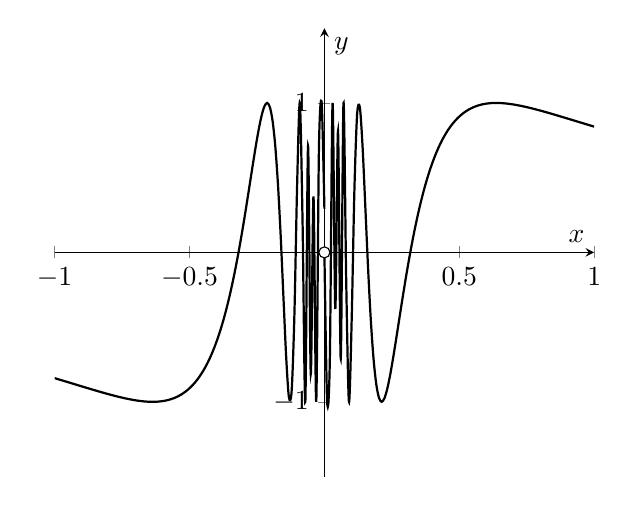
\begin{tikzpicture}
        \begin{axis}[
            axis lines = middle,
            xlabel = $x$,
            ylabel = {$y$},
            domain=-1:1,
            samples=200,
            ymin=-1.5, ymax=1.5,
            restrict y to domain=-2:2,  % To handle large values near discontinuity
            ]
            % Plot the function excluding x=0
            \addplot[
                domain=-1:-0.00001,
                samples=100,
                thick,
                smooth,
            ]{sin(deg(1/x))};
            \addplot[
                domain=0.00001:1,
                samples=100,
                thick,
                smooth,
            ]{sin(deg(1/x))};
            % Add a hole at x=0
            \addplot[
                only marks,
                mark=*,
                mark options={fill=white, draw=black},
            ] coordinates {(0, 0)};
        \end{axis}
    \end{tikzpicture}
    \caption{Plot of $y = f(x) = \sin\left(\frac{1}{x}\right)$}
    \label{fig:sinrx}
\end{figure}

As seen in Figure \ref{fig:sinrx}, $y = f(x)$ oscillates wildly. It does not even approach a value as $f(x)$ gets smaller; we will leave
the verification of this to the reader. Hence, the limit does not exist here, as $f(x)$ never converges to any
particular value.

In fact, the limit does not even need to exist. Consider the sign function $\sgn(x)$, where
$\sgn(x) = -1$ for $x < 0$, $\sgn(x) = 1$ for $x > 0$ and $\sgn(x) = 0$ for $x = 0$, and its
graph in Figure \ref{fig:sgn}.

We know that $\sgn(x)$ is defined everywhere, including $0$. However, limits study the behavior of
functions \textit{around} some point, not \textit{at} that point.

If we look from the left of Figure \ref{fig:sgn}, it seems like $\sgn(x)$ is approaching $-1$ as $x$ approaches $0$ from
$-\infty$. However, from the right, it seems like $\sgn(x)$ is approaching $1$ as $x$ approaches $0$
from $+\infty$ (the positive sign is explicitly used here to emphasize that we approach from the right).

Hence, because $\sgn(x)$ does not settle on only one value when $x$ approaches $0$ from both sides
(i.e., the values are different, as stated previously), the limit of $\sgn(x)$ as $x \to 0$ \textbf{does
not exist}.

\begin{figure}[h]
    \centering
    \begin{tikzpicture}
        \begin{axis}[
            axis lines = middle,
            xlabel = $x$,
            ylabel = {$y$},
            domain=-1:1,
            samples=200,
            ymin=-1.5, ymax=1.5,
            restrict y to domain=-2:2,  % To handle large values near discontinuity
            ]
            % Plot the function excluding x=0
            \addplot[
                domain=-1:-0.00001,
                samples=100,
                thick,
                smooth,
            ]{-1};
            \addplot[
                domain=0.00001:1,
                samples=100,
                thick,
                smooth,
            ]{1};
            % Add a hole at x=0
            \addplot[
                only marks,
                mark=*,
                mark options={fill=black, draw=black},
            ] coordinates {(0, 0)};
        \end{axis}
    \end{tikzpicture}
    \caption{Plot of $y = \sgn(x)$}
    \label{fig:sgn}
\end{figure}

\newpage

\section{Operations of limits}
Suppose that $\lim_{x \to c} f(x) = A$ and $\lim_{x \to c} g(x) = B$ for the functions $f(x)$, $g(x)$,
and $A,B$ are constants. Then:
\[
\lim_{x \to c} (f(x) \pm g(x)) = A \pm B,
\]
\[
\lim_{x \to c} (f(x) g(x)) = A B,
\]
\[
\lim_{x \to c} \left(\frac{f(x)}{g(x)}\right)  = \frac{A}{B},\,\,B\ne 0,
\]
\[
\lim_{x \to c} kf(x) = k\lim_{x \to c} f(x) = kA,\,\,k\,\,\text{is a constant.}
\]

\begin{example}
    Find the limit of $k e^{-x}$, as $x$ tends to infinity. 
\end{example}
\begin{solution}
    The limit is \[\lim_{x \to \infty} k e^{-x} = k \lim_{x \to -\infty} e^{-x} = k \times 0 = 0.\]
    One can study the behavior of $e^{-x}$ graphically.
\end{solution}

\section{The squeeze theorem}
The squeeze theorem is extremely useful in determining important limits; in fact, it is key to proving the
derivative of $\sin(x)$ (with respect to $x$). Hence, we begin with a statement of the theorem.

\begin{theorem}[Squeeze theorem]\thlabel{squeeze}
    Suppose that we have three functions $f(x), g(x), h(x)$ such that $g(x)\le f(x)\le h(x)$. Then
    \[
    \lim_{x \to c} g(x) = \lim_{x \to c} h(x) = L \implies \lim_{x \to c} f(x) = L
    \]
    where $c$ is a constant.
\end{theorem}
\begin{proof}
    The proof can be found on Wikipedia.
    % It is beyond the scope of this book.
\end{proof}

Now, we begin with some examples.

\begin{example}
    Find the limit \[\lim_{x \to 0}x^2\sin\left(\frac{1}{x}\right).\]
\end{example}
\begin{solution}
    We cannot apply the law
    \[
    \lim_{x \to c} (f(x) g(x)) = A B
    \]
    because $\lim_{x \to 0} \sin\left(\frac{1}{x}\right)$ does not exist. However, since the range of $\sin(x)$
    is $[-1, 1]$, we can establish the inequality \[-1 \le \sin\left(\frac{1}{x}\right) \le 1.\] Multiplying both
    sides by $x^2$, we obtain \[-x^2 \le x^2 \sin\left(\frac{1}{x}\right) \le x^2.\]
    Evaluating the leftmost and
    rightmost limits by direct substitution,
    \[\lim_{x \to 0} x^2 = \lim_{x \to 0} (-x^2) = 0 \implies
    \lim_{x \to 0} x^2 \sin\left(\frac{1}{x}\right) = 0 \]
    by the squeeze theorem, and we are done.
\end{solution}

\section{Differentiation from first principles}
Differentiation in the `A'-Level and `O'-Level has, in the author's experience, only been taught in terms of
memorizing formulae and identities. For example, one simply assumes that \[\frac{d}{dx}\sin(x) = \cos(x).\]

The proof of this `trivial' identity, is not `trivial'; it has never ever been covered in any
ordinary course. This is because the proof of this identity utilizes \thref{squeeze}.
In fact, most trigonometric identities stem from the aforementioned theorem.

Now, we must start with the very definition of what a
derivative is. Instead of introducing the definition directly without further explanation, let us
briefly derive the definition of the derivative ourselves.

Recall that the gradient of a straight line $y$ passing through two points $(x_1, y_1)$ and $(x_2, y_2)$ is
defined as $m = \frac{y_2 - y_1}{x_2 - x_1}.$, where $x_2 > x_1$ and $x,y \in \mathbb{R}$.
If $y = f(x)$, then $m = \frac{f(x_2) - f(x_1)}{x_2 - x_1}.$

Now, consider the difference between $x_2$ and $x_1$; let this difference be
$\delta = x_2 - x_1$. Then $x_2 = x_1 + \delta$. Replacing all such occurences of $x_2$, one obtains
\[m = \frac{f(x_1 + \delta) - f(x_1)}{\delta}.\]

We have learnt that we can draw a tangent at a point in a graph to find the gradient at that point; this is exactly
the idea we use here to formally define the derivative. As $\delta$ tends to $0$, we will get a better approximation
of the gradient at the point $(x_1, y_1)$. Alas, using limits, we have the following definition:

\begin{definition}
    The derivative of a function $f(x)$, with respect to $x$, is defined as
    \[f'(x) = \lim_{\delta \to 0} \frac{f(x + \delta) - f(x)}{\delta}\]
\end{definition}

When we apply this definition in finding a derivative, the process is dubbed as \textit{differentiating
from first principles}.

\begin{example}
    Find the derivative of $f(x) = 3x^2 + 2x + 1$.
\end{example}
\begin{solution}
    By differentiating from first principles, one obtains
    \begin{equation*}
        \begin{split}
            f'(x) &= \lim_{\delta \to 0} \frac{f(x + \delta) - f(x)}{\delta} \\
            &= \lim_{\delta \to 0} \frac{(3(x + \delta)^2 + 2(x + \delta) + 1) - (3x^2 + 2x + 1)}{\delta} \\
            &= \lim_{\delta \to 0} \frac{3(x + \delta)^2 + 2x + 2\delta + 1 - 3x^2 - 2x - 1}{\delta} \\
            &= \lim_{\delta \to 0} \frac{3(x + \delta)^2 + 2\delta - 3x^2}{\delta} \\
            &= \lim_{\delta \to 0} \frac{3(x^2 + 2x\delta + \delta^2) + 2\delta - 3x^2}{\delta} \\
            &= \lim_{\delta \to 0} \frac{3x^2 + 6x\delta + 3\delta^2 + 2\delta - 3x^2}{\delta} \\
            &= \lim_{\delta \to 0} \frac{6x\delta + 3\delta^2 + 2\delta}{\delta} \\
            &= \lim_{\delta \to 0} 6x + 3\delta + 2 \\
            &= 6x + 3(0) + 2 \\
            &= 6x + 2
        \end{split}
    \end{equation*}
    Indeed, this is what we expect since \[\frac{d}{dx}(3x^2 + 2x + 1) = 6x + 2.\]
    Hence we are done.
\end{solution}

\section{L'H\^{o}pital's rule}
L'H\^{o}pital's rule is a theorem popularly used to evaluate limits of expressions which take,
after direct substitution, $\frac{f(x)}{g(x)} = \frac{0}{0}$ or $\frac{\infty}{\infty}$.
If we assume that $f(x)$ and $g(x)$ are differentiable everywhere, and they are well defined
everywhere, we state L'H\^{o}pitals rule as follows:

\begin{theorem}[L'H\^{o}pital's rule]
    For any functions $f : \mathbb{R} \to \mathbb{R}$ and $g : \mathbb{R} \to \mathbb{R}$ differentiable everywhere and well-defined
    everywhere,
    \[\lim_{x \to c} \frac{f(x)}{g(x)} = \lim_{x \to c} \frac{f'(x)}{g'(x)}\]
    if the following conditions hold:
    \begin{itemize}
        \item $\lim_{x \to c} f(x) = \lim_{x \to c} g(x) = 0 \,\,\text{or}\,\pm \infty$
        \item $g'(x) \ne 0$
        \item $\lim_{x \to c} \frac{f'(x)}{g'(x)}$ exists
    \end{itemize}
    where $f(x),g(x)$ are functions of $x$.
\end{theorem}

\newpage
\section{Exercises}

\begin{exercise}
    approximate the limit of $\frac{1}{x}$ as $x$ approaches $0$ from both sides
    (i.e., approximate the left and right limits). Hence, explain why
    \[\lim_{x \to 0} \frac{1}{x}\]
    does not exist.
\end{exercise}

\begin{exercise}
    Prove that \[\lim_{x \to 0} |f(x)| = 0 \implies \lim_{x \to 0} f(x) = 0\]
    using the squeeze theorem. (Hint: $|-f(x)| = |f(x)|$. Form an inequality.)
\end{exercise}

\begin{exercise}
    It is known that the sum of a geometric series up to $n$ terms is given by
    \[S_n = \sum_{k=1}^n ar^{k - 1} = \frac{a(r^n - 1)}{r - 1}\]
    If $|r| < 0$, take the limit of $S_n$ as $n$ approaches $\infty$.
\end{exercise}

\backmatter

\bibliographystyle{plain}
\bibliography{refs}

\end{document}